\documentclass[]{article}
\usepackage[margin=2cm]{geometry}

%opening
\title{Exercises Set: Calculus}
\author{DSBA Mathematics Refresher 2025}
\date{}

\usepackage{amsmath}
\usepackage{amsfonts}
\usepackage{amsthm}
\usepackage{amssymb}
\usepackage{mathrsfs}
\usepackage{stmaryrd}
\usepackage{tikz}

\newcommand{\Q}{\mathbb{Q}}
\newcommand{\N}{\mathbb{N}}
\newcommand{\Z}{\mathbb{Z}}
\newcommand{\R}{\mathbb{R}}
\newcommand{\Primes}{\mathbb{P}}
\newcommand{\st}{\text{ s.t. }}
\newcommand{\txtand}{\text{ and }}
\newcommand{\txtor}{\text{ or }}
\newcommand{\lxor}{\veebar}


\begin{document}

	\maketitle
	
	\begin{abstract}
		Only the questions with a * are compulsory (but do all of them!).
	\end{abstract}
	
	\section{Fundamental Theorem of Calculus}
	\paragraph{Statement}\mbox{}\\
	Let $f$ be a continuous real-valued function defined on a closed interval $\left[ 0,x \right]$.
	Let $F$ be the function defined, for all $t \in \left[ 0,x \right]$, by $F(x) = \int_0^x f(t) dt$.
	
	Then $F$ is uniformly continuous on $\left[ 0,x \right]$ and differentiable on the open interval $\left( a,b \right)$, and $F'(x) = f(x)$ for all $x \in \left( a,b \right)$ so $F$ is an anti-derivative of $f$.
	
	\paragraph{Generalization / Corollary}\mbox{}\\
	Let \( f(x) \) be a continuous function on the closed interval \([a, b] \ni  0 \), and let \( F \) be an anti-derivative of \( f \).
	Prove that
	\[
	\int_a^b f(x) \, dx = F(b) - F(a).
	\]
	
	\paragraph{Application}\mbox{}\\
	Evaluate the following definite integral using the Fundamental Theorem of Calculus:
	\[
	\int_0^{\pi/2} \sin(x) \, dx
	\]
	
	Evaluate the following definite integral using the Fundamental Theorem of Calculus:
	\[
	\int_1^4 \frac{1}{x^2} \, dx
	\]
	
	
	\section{Integration Techniques}
	\paragraph{Reminder}
	$$\int f(u) \, du = \int f(g(x)) \cdot g'(x) \, dx \quad \text {or} \quad \int f(u) \, du = \int f(x) \cdot \frac{du}{dx} \, dx$$
	$$\int u v' = uv - \int v u'$$
	
	\paragraph{Substitution / Change of Variable}\mbox{}
	
	
	\textbf{Exercise 1:}
	Evaluate the following integral using the method of substitution:
	\[
	\int \frac{2x}{x^2 + 1} \, dx
	\]
	\textit{Hint:} Let \( u = x^2 + 1 \) and then find \( du \) to perform the substitution.
	
	\textbf{Exercise 2: (*)}
	Evaluate the following integral using the method of substitution:
	\[
	\int \frac{1}{\sqrt{1 - x^2}} \, dx
	\]
	\textit{Hint:} Let \( x = \sin(u) \) and then find \( du \) to perform the substitution.
	
	\textbf{Exercise 3:}
	Evaluate the following integral using a trigonometric substitution:
	\[
	\int \frac{1}{4 + x^2} \, dx
	\]
	\textit{Hint:} Use the substitution \(u = x/2\) to simplify the integral.
	
	
	\paragraph{Integration by Parts}\mbox{}
	
	\textbf{Exercise A:}
	Compute the following integral using integration by parts:
	\[
	\int x \ln(x) \, dx
	\]
	
	\textbf{Exercise B:}
	Find the value of the integral using integration by parts:
	\[
	\int x^2 e^x \, dx
	\]
	
	\textbf{Exercise C: (*)}
	Compute the following integral using integration by parts:
	\[
	\int x \cos(x) \, dx
	\]
	
	\textbf{Exercise D:}
	Evaluate the following integral using the method of substitution:
	\[
	\int e^{2x} \cos(2x) \, dx
	\]
	
	
	\paragraph{Further integration techniques}\mbox{}
	
	\textbf{Exercise $\alpha$:}
	Decomposing the fraction of the following expression:
	\[
	\frac{3x^2 - 2x - 1}{x^3 - x^2 + x - 1}
	\]
	Calculate
	\[
	\int \frac{3x^2 - 2x - 1}{x^3 - x^2 + x - 1} dx
	\]
	\textit{Hint:} Factor the numerator and denominator.
	
	\textbf{Exercise $\beta$: (*)}
	Evaluate the following improper integral by decomposition:
	\[
	\int_0^{+\infty} e^{-x}\, dx
	\]
	\textit{Hint:} Evaluate the improper integral by considering the limits is $a$, and let $a$ approach infinity.
	
	\textbf{Exercise $\gamma$:}
	Approximate the value of the integral
	\[
	\int_0^{\pi/2} \sin(x) \, dx
	\]
	using the Trapezoidal Rule with \(n = 3\) sub-intervals.
	
	\textbf{Exercise $\delta$:}
	Estimate the value of the integral
	\[
	\int_0^{\pi/2} \sin(x) \, dx
	\]
	using Simpson's Rule with \(n = 2\) sub-intervals.
	
	
	\section{Applications}
	\paragraph{Areas between curves}\mbox{}\\
	Determine the area of the region enclosed by the curves \(y = \sin(x)\) and \(y = -\sin(x)\) over the interval \([0, \pi]\).\\
	\textit{Hint:} Begin by finding the points of intersection between the two curves within the given interval.
	Then, set up the integral to calculate the area between the curves.
	\begin{center}
		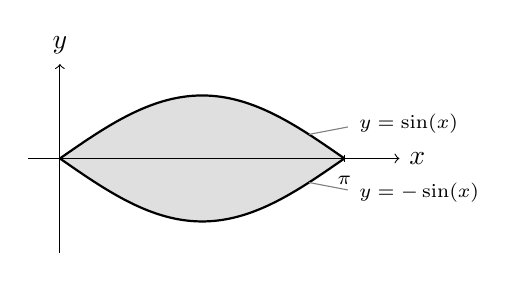
\begin{tikzpicture}[xscale=1.15,yscale=0.8]
			\fill[gray!25] plot[domain=0:pi,samples=100,smooth] (\x,{sin(\x r)}) -- plot[domain=pi:0,samples=100,smooth] (\x,{-sin(\x r)}) -- cycle;
			\draw[->] (-0.35,0) -- (3.75,0) node[right] {$x$};
			\draw[->] (0,-1.5) -- (0,1.5) node[above] {$y$};
			\draw[thick,domain=0:pi,samples=100,smooth] plot (\x,{sin(\x r)});
			\draw[thick,domain=0:pi,samples=100,smooth] plot (\x,{-sin(\x r)});
			\draw (pi,0.06) -- (pi,-0.06); \node[below] at (pi,-0.12) {\scriptsize $\pi$};
			\node[right] at (3.2,0.55) {\scriptsize $y=\sin(x)$};
			\node[right] at (3.2,-0.55) {\scriptsize $y=-\sin(x)$};
			\draw[gray] (3.18,0.5) -- (2.75,{sin(2.75 r)});
			\draw[gray] (3.18,-0.5) -- (2.75,{-sin(2.75 r)});
		\end{tikzpicture}
	\end{center}
	
	\paragraph{Volume of a solid of revolution (*)} (Disk Method)\\
	Find the volume of the solid generated by revolving the region bounded by \(y = x^2\) and the $y$-axis, over the interval \( y\in [0, 1] \), about the $y$-axis using the disk method.\\
	\textit{Hint:} Determine the limits of integration, the radius of the disks, and set up the integral to find the volume.
	\begin{center}
		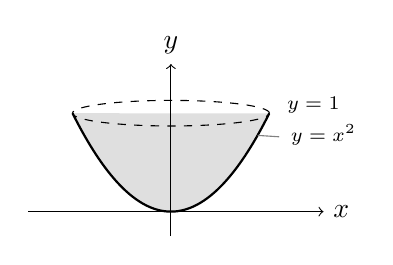
\begin{tikzpicture}[scale=1.25]
			\fill[gray!25] plot[domain=-1:1,samples=100,smooth] (\x,{\x*\x}) -- cycle;
			\draw[->] (-1.45,0) -- (1.55,0) node[right] {$x$};
			\draw[->] (0,-0.25) -- (0,1.5) node[above] {$y$};
			\draw[thick,domain=-1:1,samples=100,smooth] plot (\x,{\x*\x});
			\draw[dashed] (0,1) ellipse (1 and 0.13);
			\node[right] at (1.08,1.08) {\scriptsize $y=1$};
			\node[right] at (1.12,0.78) {\scriptsize $y=x^2$};
			\draw[gray] (1.10,0.76) -- (0.88,{0.88*0.88});
		\end{tikzpicture}
	\end{center}
	
	\paragraph{Arc length of curves}\mbox{}\\
	Find the arc length of the curve defined by \(y = \frac{2}{3} x\sqrt{x}\) over the interval \([0, 3]\).\\
	\textit{Hint:} Use the formula for arc length \(\int_a^b \sqrt{1 + (f'(x))^2} \, dx\) to calculate the arc length of the curve.
	The coefficient \(\frac{2}{3}\) has been chosen to make \(1 + (f'(x))^2\) as simple as possible.
	\begin{center}
		\begin{tikzpicture}[xscale=1.0,yscale=0.6]
			\draw[->] (-0.3,0) -- (3.75,0) node[right] {$x$};
			\draw[->] (0,-0.3) -- (0,3.85) node[above] {$y$};
			\draw[thick,domain=0:3,samples=100,smooth] plot (\x,{2/3*pow(\x,1.5)});
			\draw (3,0.08) -- (3,-0.08); \node[below] at (3,-0.05) {\scriptsize $3$};
			\node[right] at (2.2,1.35) {\scriptsize $y=\frac{2}{3}x\sqrt{x}$};
			\draw[gray] (2.18,1.4) -- (1.85,{2/3*pow(1.85,1.5)});
		\end{tikzpicture}
	\end{center}
	
	\paragraph{Surface area of a solid of revolution}\mbox{}\\
	Find the surface area of the solid generated by revolving the curve \(y = x^2\) over the interval \( y \in [0, 2] \) about the $y$-axis.\\
	\textit{Hint:} The area is \(\int 2\pi \, r \, ds\), where $r$ is the distance to the axis of revolution and \(ds = \sqrt{1 + (f'(x))^2} \, dx\) is the arc length element --- \textit{not} $dx$ or $dy$, as a strip of the surface is slanted.
	Integrating with respect to $y$ makes the computation particularly short here.
	\begin{center}
		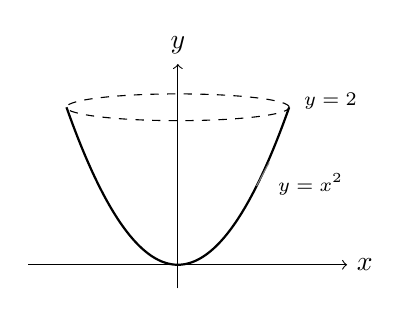
\begin{tikzpicture}[scale=1.0]
			\draw[->] (-1.9,0) -- (2.15,0) node[right] {$x$};
			\draw[->] (0,-0.3) -- (0,2.55) node[above] {$y$};
			\draw[thick,domain=-1.4142:1.4142,samples=100,smooth] plot (\x,{\x*\x});
			\draw[dashed] (0,2) ellipse (1.4142 and 0.17);
			\node[right] at (1.48,2.08) {\scriptsize $y=2$};
			\node[below right] at (1.15,1.28) {\scriptsize $y=x^2$};
			\draw[gray] (1.16,1.3) -- (1.0,1.0);
		\end{tikzpicture}
	\end{center}
	

\end{document}
